\documentclass{beamer}

\usepackage[utf8]{inputenc} % Language and font encoding
\usepackage[icelandic]{babel}
\usepackage[T1]{fontenc}


\usepackage{tikz}
\usepackage[listings,theorems]{tcolorbox}
\usepackage{booktabs}
\usepackage{minted} %Minted and configuration
\usemintedstyle{default}

\renewcommand{\theFancyVerbLine}{\sffamily \arabic{FancyVerbLine}}
%%%%%%%%%%%
% More math
%%%%%%%%%%%
\newcommand{\Mod}[1]{\ \text{mod}\ #1}

%%%%%%%%%%%%%%%%%%%%%%
% Beamer configuration
%%%%%%%%%%%%%%%%%%%%%%
\setbeamertemplate{navigation symbols}{}
\usecolortheme{dove}
\setbeamercolor{frametitle}{fg=white}

\usebackgroundtemplate%
{%
\vbox to \paperheight{

\includegraphics[width=\paperwidth]{Pics/hi-slide-head-2016}

\vfill
\hspace{0.5cm}
\includegraphics[width=0.3\paperwidth]{Pics/hi-von-logo}
\vspace{0.4cm}
    }%
}

\AtBeginSection[]
{
  \begin{frame}<beamer>
    \frametitle{Yfirlit}
    \tableofcontents[currentsection]
  \end{frame}
}

\setbeamerfont{frametitle}{size=\normalsize}
\addtobeamertemplate{frametitle}{}{\vspace*{0.5cm}}

%%%%%%%%%%%%%%%%%%%%%%%%%
% tcolorbox configuration
%%%%%%%%%%%%%%%%%%%%%%%%%

% Setup from: http://tex.stackexchange.com/a/43329/21638
\tcbset{%
    noparskip,
    colback=gray!10, %background color of the box
    colframe=gray!40, %color of frame and title background
    coltext=black, %color of body text
    coltitle=black, %color of title text 
    fonttitle=\bfseries,
    alerted/.style={coltitle=red, colframe=gray!40},
    example/.style={coltitle=black, colframe=green!20, colback=green!5},
}


%%%%%%%%%%%%%%%%%%%%%%%
% Further configuration
%%%%%%%%%%%%%%%%%%%%%%%
\hypersetup{colorlinks=true,pdfauthor={Eirikur Ernir Thorsteinsson},linkcolor=blue,urlcolor=blue}
\graphicspath{{./Pics/}}

\author{Eiríkur Ernir Þorsteinsson}
\institute{Háskóli Íslands}
\date{Haust 2016}

\title{Stærðfræðimynstur í tölvunarfræði}
\subtitle{Vika 11, seinni fyrirlestur}

\begin{document}

\begin{frame}
\titlepage
\end{frame}


\section{Inngangur}

\begin{frame}{Í síðasta tíma}
\begin{itemize}
 \item Um misserislok
 \item Vegir 
 \item Samanhangandi net
\end{itemize}
\end{frame}

\section{Euler-vegir}

\begin{frame}{Elsta netavandamálið}
Í borginni Königsberg voru eitt sinn 7 brýr.
\begin{center}
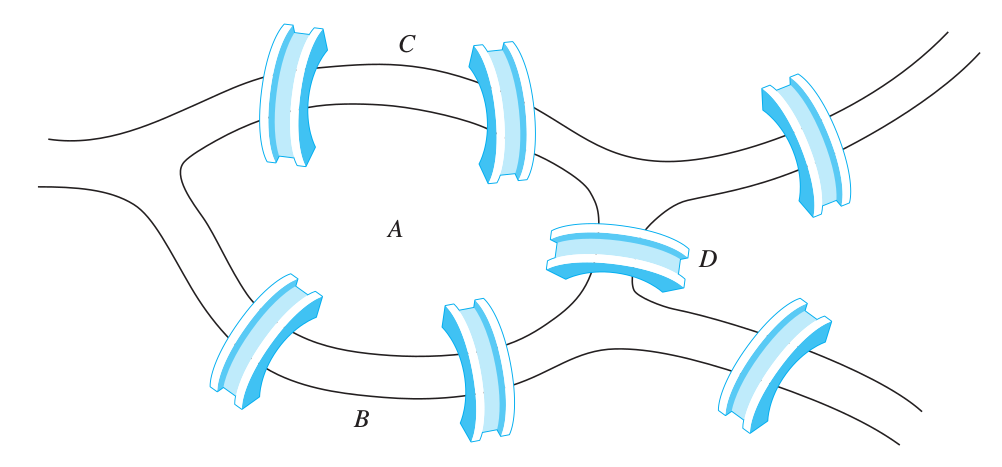
\includegraphics[width=0.8\textwidth]{konigsberg}
\end{center}
Er hægt að fara í göngutúr sem endar á sama stað og hann byrjar og liggur yfir hverja brú nákvæmlega einu sinni?
\end{frame}

\begin{frame}{Netaframsetning}
\begin{columns}
\column{0.6\textwidth}
Stærðfræðingurinn Leonhard Euler leysti vandamálið með netaframsetningu.

Við getum skilgreint Euler-rás:

\begin{tcolorbox}[title=Euler-rás]
Euler-rás (e. \emph{Euler circuit}) í óstefndu neti $G$ er einföld rás sem inniheldur alla leggi í $G$.
\end{tcolorbox}
Er til Euler-rás í Königsberg-netinu?
\column{0.4\textwidth}
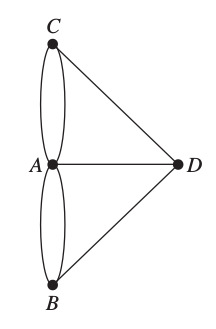
\includegraphics[width=\textwidth]{konigsberg-graph}
\end{columns}
\end{frame}

\begin{frame}{Euler-rásir}
Við getum fundið skilyrði sem er nauðsynlegt og nægjanlegt fyrir tilvist Euler-rásar í óstefndu neti.

\begin{tcolorbox}
Samanhangandi óstefnt net með a.m.k. tveimur hnútum hefur Euler-rás ef og aðeins ef stig allra hnúta í netinu er slétt tala.
\end{tcolorbox}

Königsberg-göngutúrinn okkar er þá ekki mögulegur.
\end{frame}

\begin{frame}{Að finna Euler-rásir}
\begin{center}
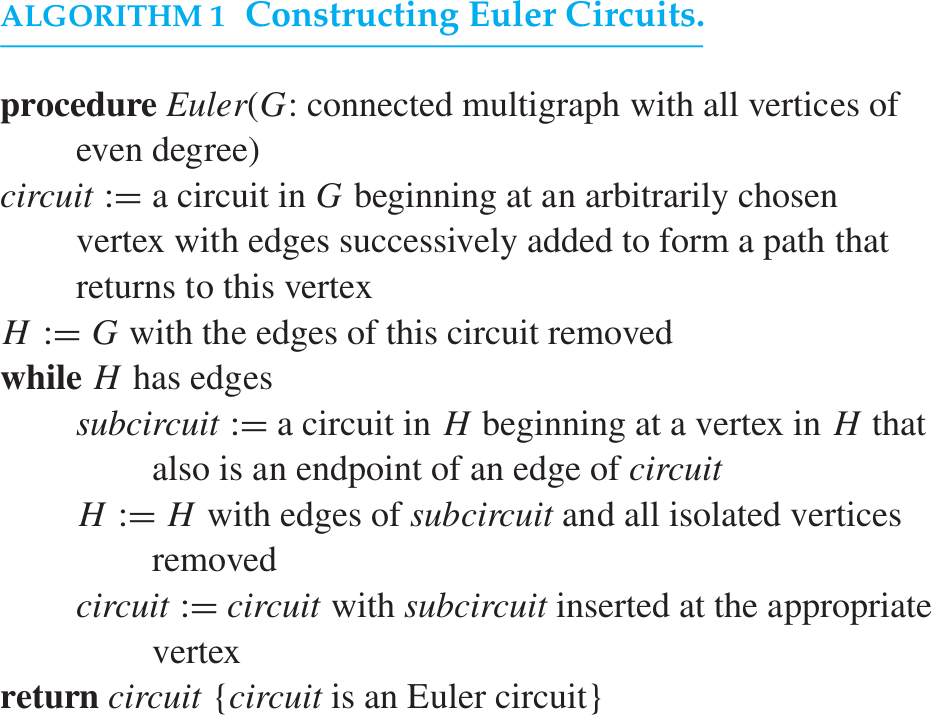
\includegraphics[width=0.8\textwidth]{finding-euler}
\end{center}
\end{frame}

\begin{frame}{Dæmi}
Við getum fundið Euler-rás í þessu neti.
\begin{center}
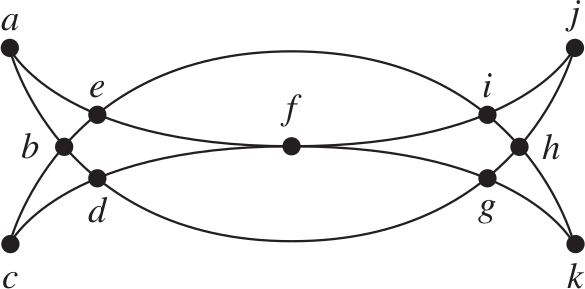
\includegraphics[width=0.6\textwidth]{mohammed-scimitars}
\end{center}
\pause
Möguleg lausn:
\[
a, b, d, g, h, j, i, h, k, g, f, d, c, b, e, i, f, e, a
\]

\end{frame}

\begin{frame}{Euler-vegir}
\begin{tcolorbox}[title=Euler-vegur]
Euler-vegur (e. \emph{Euler path}) í óstefndu neti $G$ er einfaldur vegur sem inniheldur alla leggi í $G$.
\end{tcolorbox}

\begin{tcolorbox}
Samanhangandi óstefnt net hefur Euler-veg ef og aðeins ef stig nákvæmlega tveggja hnúta í netinu er oddatala.
\end{tcolorbox}
\end{frame}

\section{Hamilton-vegir}

\begin{frame}{Hamilton- vegir og rásir}
\begin{tcolorbox}[title=Hamilton-vegir og rásir]
Einfaldur vegur í óstefndu neti sem fer í gegnum hvern hnút nákvæmlega einu sinni er kallaður Hamilton-vegur (e. \emph{Hamilton path}). Einföld rás sem fer nákvæmlega einu sinni í gegnum hvern hnút netsins er kölluð Hamilton-rás (e. \emph{Hamilton circuit}).
\end{tcolorbox}
\end{frame}

\begin{frame}{Dæmi}
\begin{columns}
\column{0.5\textwidth}
``Heimsferðalag'' Hamiltons

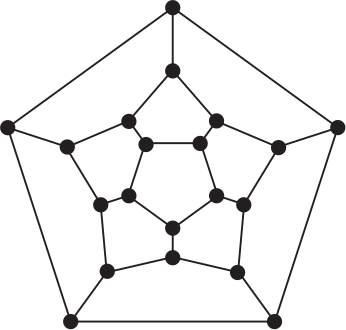
\includegraphics[width=\textwidth]{graph-hamilton}
\pause
\column{0.5\textwidth}
Netið inniheldur Hamilton-rás

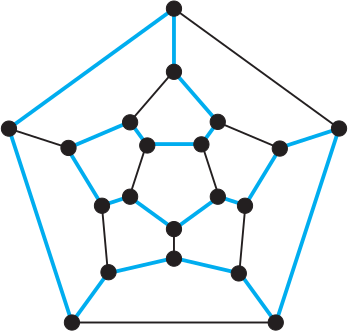
\includegraphics[width=\textwidth]{graph-hamilton-solution}
\end{columns}
\end{frame}

\begin{frame}{Dæmi}
Innihalda þessi net Hamilton-rásir? En Hamilton-vegi?
\begin{center}
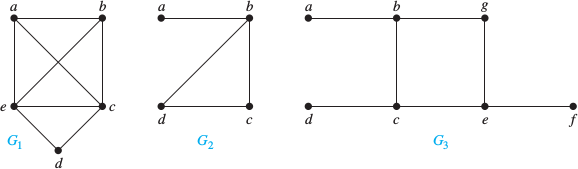
\includegraphics[width=\textwidth]{graph-hamilton-examples}
\end{center}

\end{frame}


\begin{frame}{Leitin að Hamilton-vegum}
\begin{itemize}
 \item Getum við fundið einfalda leið til að athuga hvort að gefið net innihaldi Hamilton-rás? \pause
 \begin{itemize}
  \item Engin slík leið er þekkt
 \end{itemize}
 \item 
 \item Nokkur nægjanleg skilyrði eru þekkt
 \item Engin skilyrði sem eru bæði nauðsynleg og nægjanleg eru þekkt
\end{itemize}
\end{frame}

\begin{frame}{Einfaldar staðhæfingar um Hamilton-rásir}
\begin{itemize}[<+->]
 \item Net sem inniheldur hnút af stigi 1 inniheldur ekki Hamilton-rás
 \item Hafi hnútur í neti stigið 2 hljóta báðir leggirnir sem snerta hnútinn að vera hluti af Hamilton-rás í netinu (sé slík til)
 \item Fullskipaða netið $K_n$ með $n \geq 3$ inniheldur Hamilton-rás
\end{itemize}
\end{frame}

\begin{frame}{Setningar}
\begin{tcolorbox}[title=Setning Diracs]
Sé stig allra hnúta í einföldu óstefndu neti með $n \geq 3$ hnútum a.m.k. $\frac{n}{2}$ hefur netið Hamilton-rás.
\end{tcolorbox}
\begin{tcolorbox}[title=Setning Ores]
Látum $G$ vera einfalt óstefnt net með $n \geq 3$ hnúta. Gildi að $\deg(u) + \deg(v) \geq n$ fyrir sérhverja óaðlæga hnúta $u$ og $v$ í $G$, þá hefur netið Hamilton-rás.
\end{tcolorbox}
\end{frame}

\begin{frame}{Hagnýtingar}
\begin{itemize}
 \item Hægt er að leysa alls kyns vandamál með því að setja þau fram sem leit að Hamilton-rás
 \begin{itemize}
  \item Frægt $NP$-complete vandamál
 \end{itemize}
 \item Praktísk dæmi
 \begin{itemize}
  \item Sorphirða, póstútburður\ldots
  \item Rafrásasmíði
 \end{itemize}
\end{itemize}
\end{frame}


\section{Leit að stystu vegum}

\begin{frame}{Vegin net}
Við getum geymt meiri upplýsingar í neti með því að ákvarða tölu fyrir hvern legg í netinu.
\begin{center}
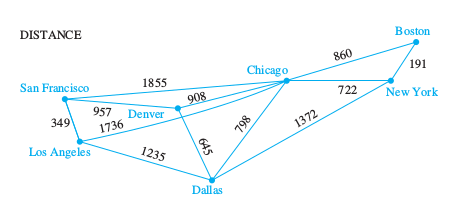
\includegraphics[width=0.7\textwidth]{graph-weighted}
\end{center}
Slíkt net er kallað vegið net (e. \emph{weighted graph}).
\end{frame}

\begin{frame}{Hagnýtingar}
\begin{itemize}
 \item Látum vegið net tákna vegakerfi þar sem þyngd leggja táknar fjarlægð milli borga
 \begin{itemize}
  \item Hver er léttasta leiðin á milli tveggja borga?
  \item Hver er léttasta leiðin sem tekur til allra borganna og endar á sama stað og hún byrjaði á?
 \end{itemize}
 \item Látum vegið net tákna rafmagnsdreifikerfi þar sem þyngd leggja táknar burðargetu rafmagnslína
 \begin{itemize}
  \item Hver er heildarburðargeta kerfisins?
  \item Hvaða kafli er mest veikburða?
 \end{itemize}
\end{itemize}
\end{frame}

\begin{frame}{Dæmi}
\begin{columns}
\column{0.6\textwidth}
Hver er léttasta leiðin á milli hnútanna $a$ og $z$?
\begin{center}
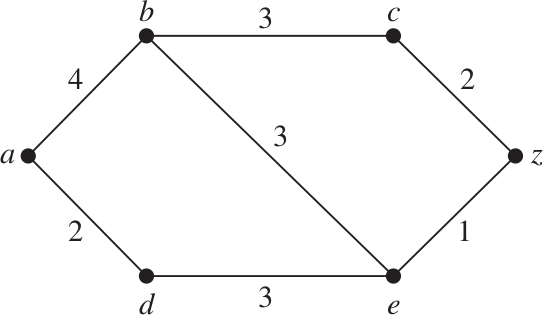
\includegraphics[width=\textwidth]{shortest-path-example}
\end{center}
\column{0.4\textwidth}
\begin{itemize}
 \item Getum leitað skipulega
 \item Finnum endurtekið léttustu leið á milli $a$ og hnúts sem við höfum ekki skoðað áður þar til við höfum fundið léttustu leið að $z$
\end{itemize}
\end{columns}
\end{frame}

\begin{frame}{Dæmi}
\begin{columns}
\column{0.6\textwidth}
Hver er léttasta leiðin á milli hnútanna $a$ og $z$?
\begin{center}
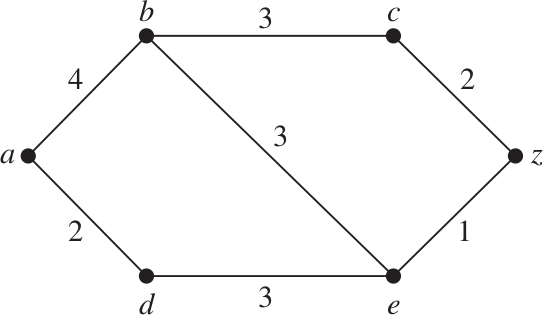
\includegraphics[width=\textwidth]{shortest-path-example}
\end{center}
\column{0.4\textwidth}
\begin{itemize}
 \item Fjarlægð 1:
 \begin{itemize}
  \item $a, d$: þyngd 2
  \item $a, b$: þyngd 4
 \end{itemize} \pause
 \item Fjarlægð 2:
 \begin{itemize}
  \item $a, b, c$: þyngd 7
  \item $a, d, e$: þyngd 5
  \item $a, b, e$: þyngd 7
 \end{itemize} \pause
 \item Fjarlægð 3:
 \begin{itemize}
  \item $a, d, c, z$: þyngd 9
  \item $a, d, e, z$: þyngd 6
 \end{itemize}
 \item Búin að skoða allt, léttasta leiðin hefur þyngdina 6
\end{itemize}
\end{columns}
\end{frame}

\begin{frame}{Reiknirit Dijkstras}
\begin{center}
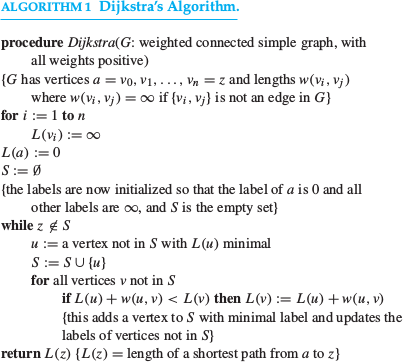
\includegraphics[width=0.8\textwidth]{dijkstras-algorithm}
\end{center}
\end{frame}

\begin{frame}{Dæmi}
\begin{center}
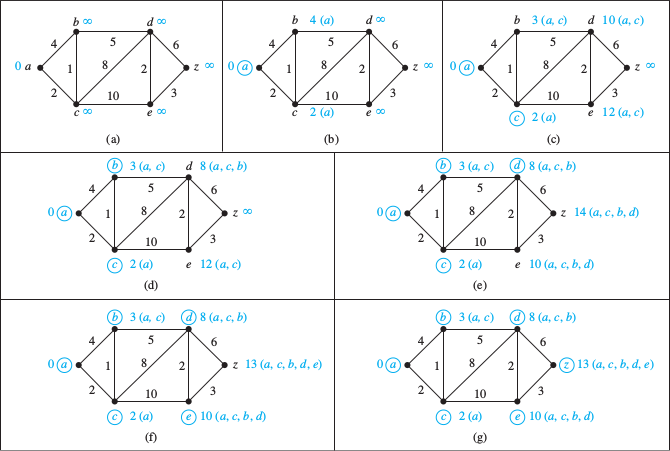
\includegraphics[width=\textwidth]{dijkstra-example}
\end{center}
\end{frame}

\section{Farandssöluvandamálið}

\begin{frame}{Farandssöluvandamálið}
\begin{itemize}
 \item Farandssöluvandamálið (e. \emph{The Traveling Salesperson Problem} eða \texttt{TSP}) er líklega frægasta netavandamálið
 \item Spurt er: Hver er léttasta rás í óstefndu, vegnu, fullskipuðu neti? \pause
 \begin{itemize}
  \item Einfaldasta leiðin: Finna allar Hamilton-rásir í netinu til að ákvarða þá stystu
  \item Vandamál: Í fullskipuðu neti eru $(n-1)!$ möguleikar á að mynda Hamilton-rás
  \begin{itemize}
   \item Hamilton-rásir eru eins í báðar áttir, þurfum að skoða $\frac{(n-1)!}{2}$ möguleika
   \item Ekki praktískt
  \end{itemize}
 \end{itemize}
 \item Þetta vandamál er $NP$-erfitt (e. \emph{NP-hard})
 \item Í alvörunni notum við nálgunarreiknirit (e. \emph{approximation algorithms}) eða brjóstvitsaðferðir (e. \emph{heuristic algorithms})
\end{itemize}
\end{frame}


\begin{frame}{Næst}
Lagnet (kafli 10.7) og litun neta (kafli 10.8).
\end{frame}


\end{document}
